\documentclass[a4paper]{article}

\usepackage[utf8]{inputenc}
\usepackage{microtype}
\usepackage{enumitem}
\usepackage{comment}
\usepackage{float, graphicx}
\usepackage{mathtools, amssymb}
\usepackage{caption}
\usepackage{subcaption}

\setlength{\parindent}{0em}


\title{2}
\date{}
\graphicspath{ {../images} }
\begin{document}
\maketitle

\section{Ideal Low Pass filter}
In order to create an ideal low-pass filter in Matlab, we created an empty image of the same dimension as the original image. And filled the middle circular region with ones ($H(u,v) = 1 if u^2 + v^2 <=D^2$). This work as our filter in the Fourier domain.

After appropriately padding both the original image and the filter, we calculated the Fourier transform of the image followed by performing a fftshift.
We then, point-wise multiplied the two images to receive the Fourier transform of the filtered image. After an ifftshift and ifft, we obtained the final filtered image. The output is:

\begin{figure}[h]
    \centering
    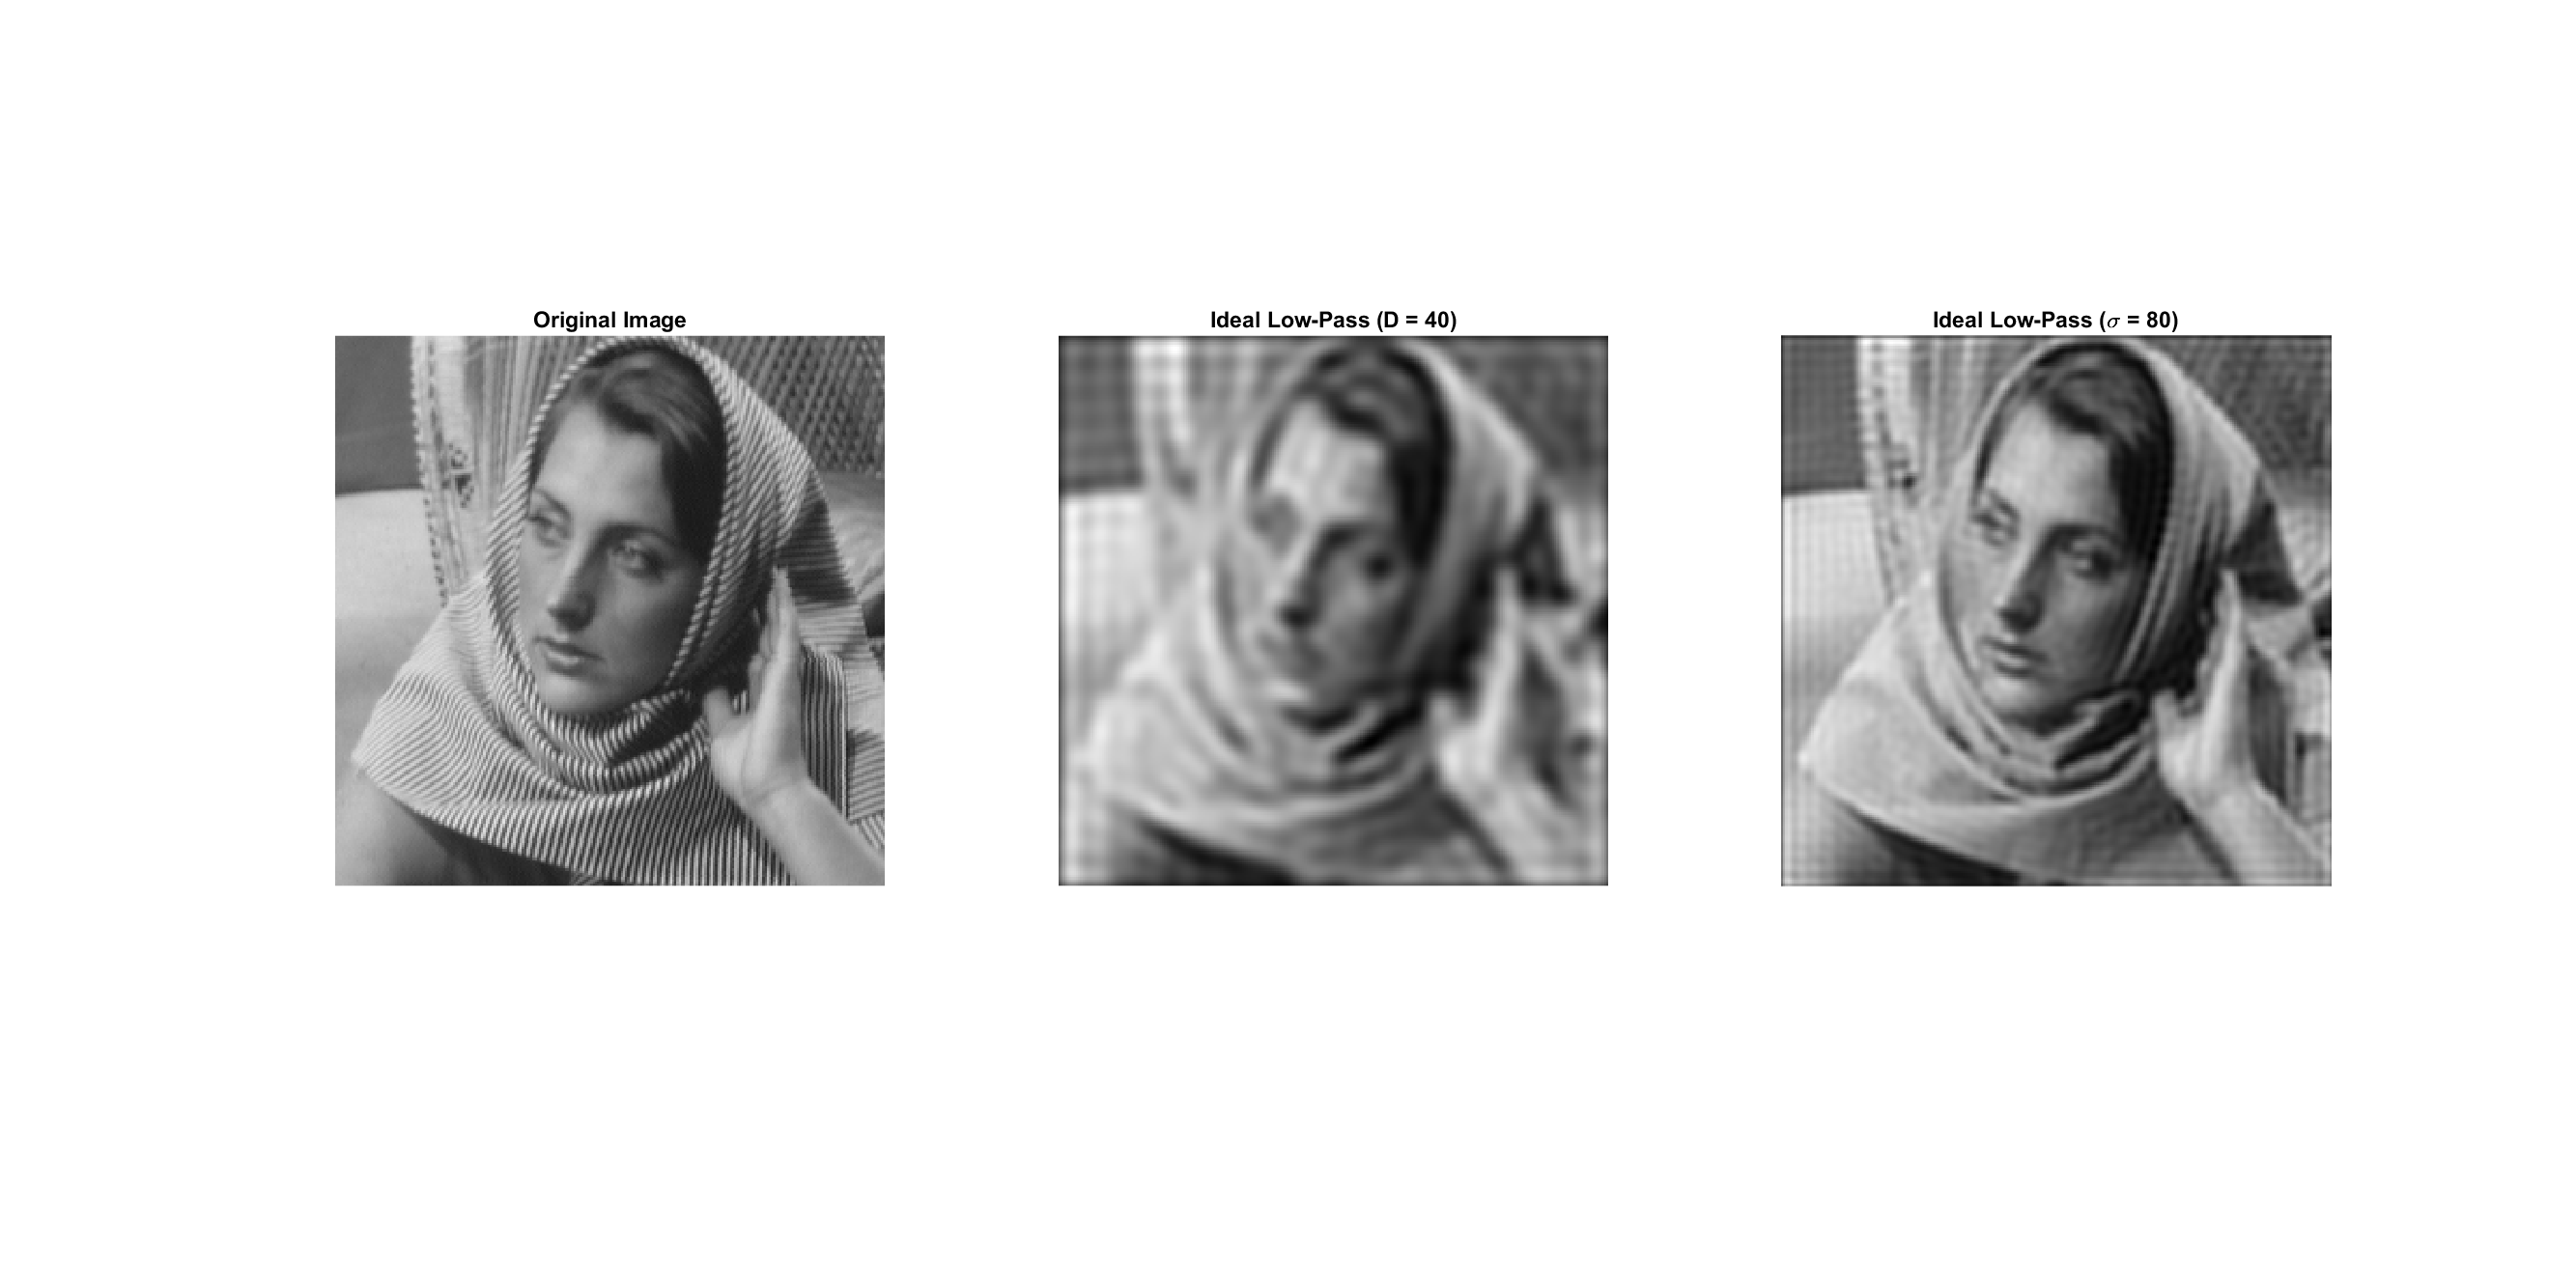
\includegraphics[width=\linewidth]{img1.png}
    \caption{Original and Filtered Images}
\end{figure}

The frequency response of the filter is((in log absolute Fourier format)):
\begin{figure}[h]
    \centering
    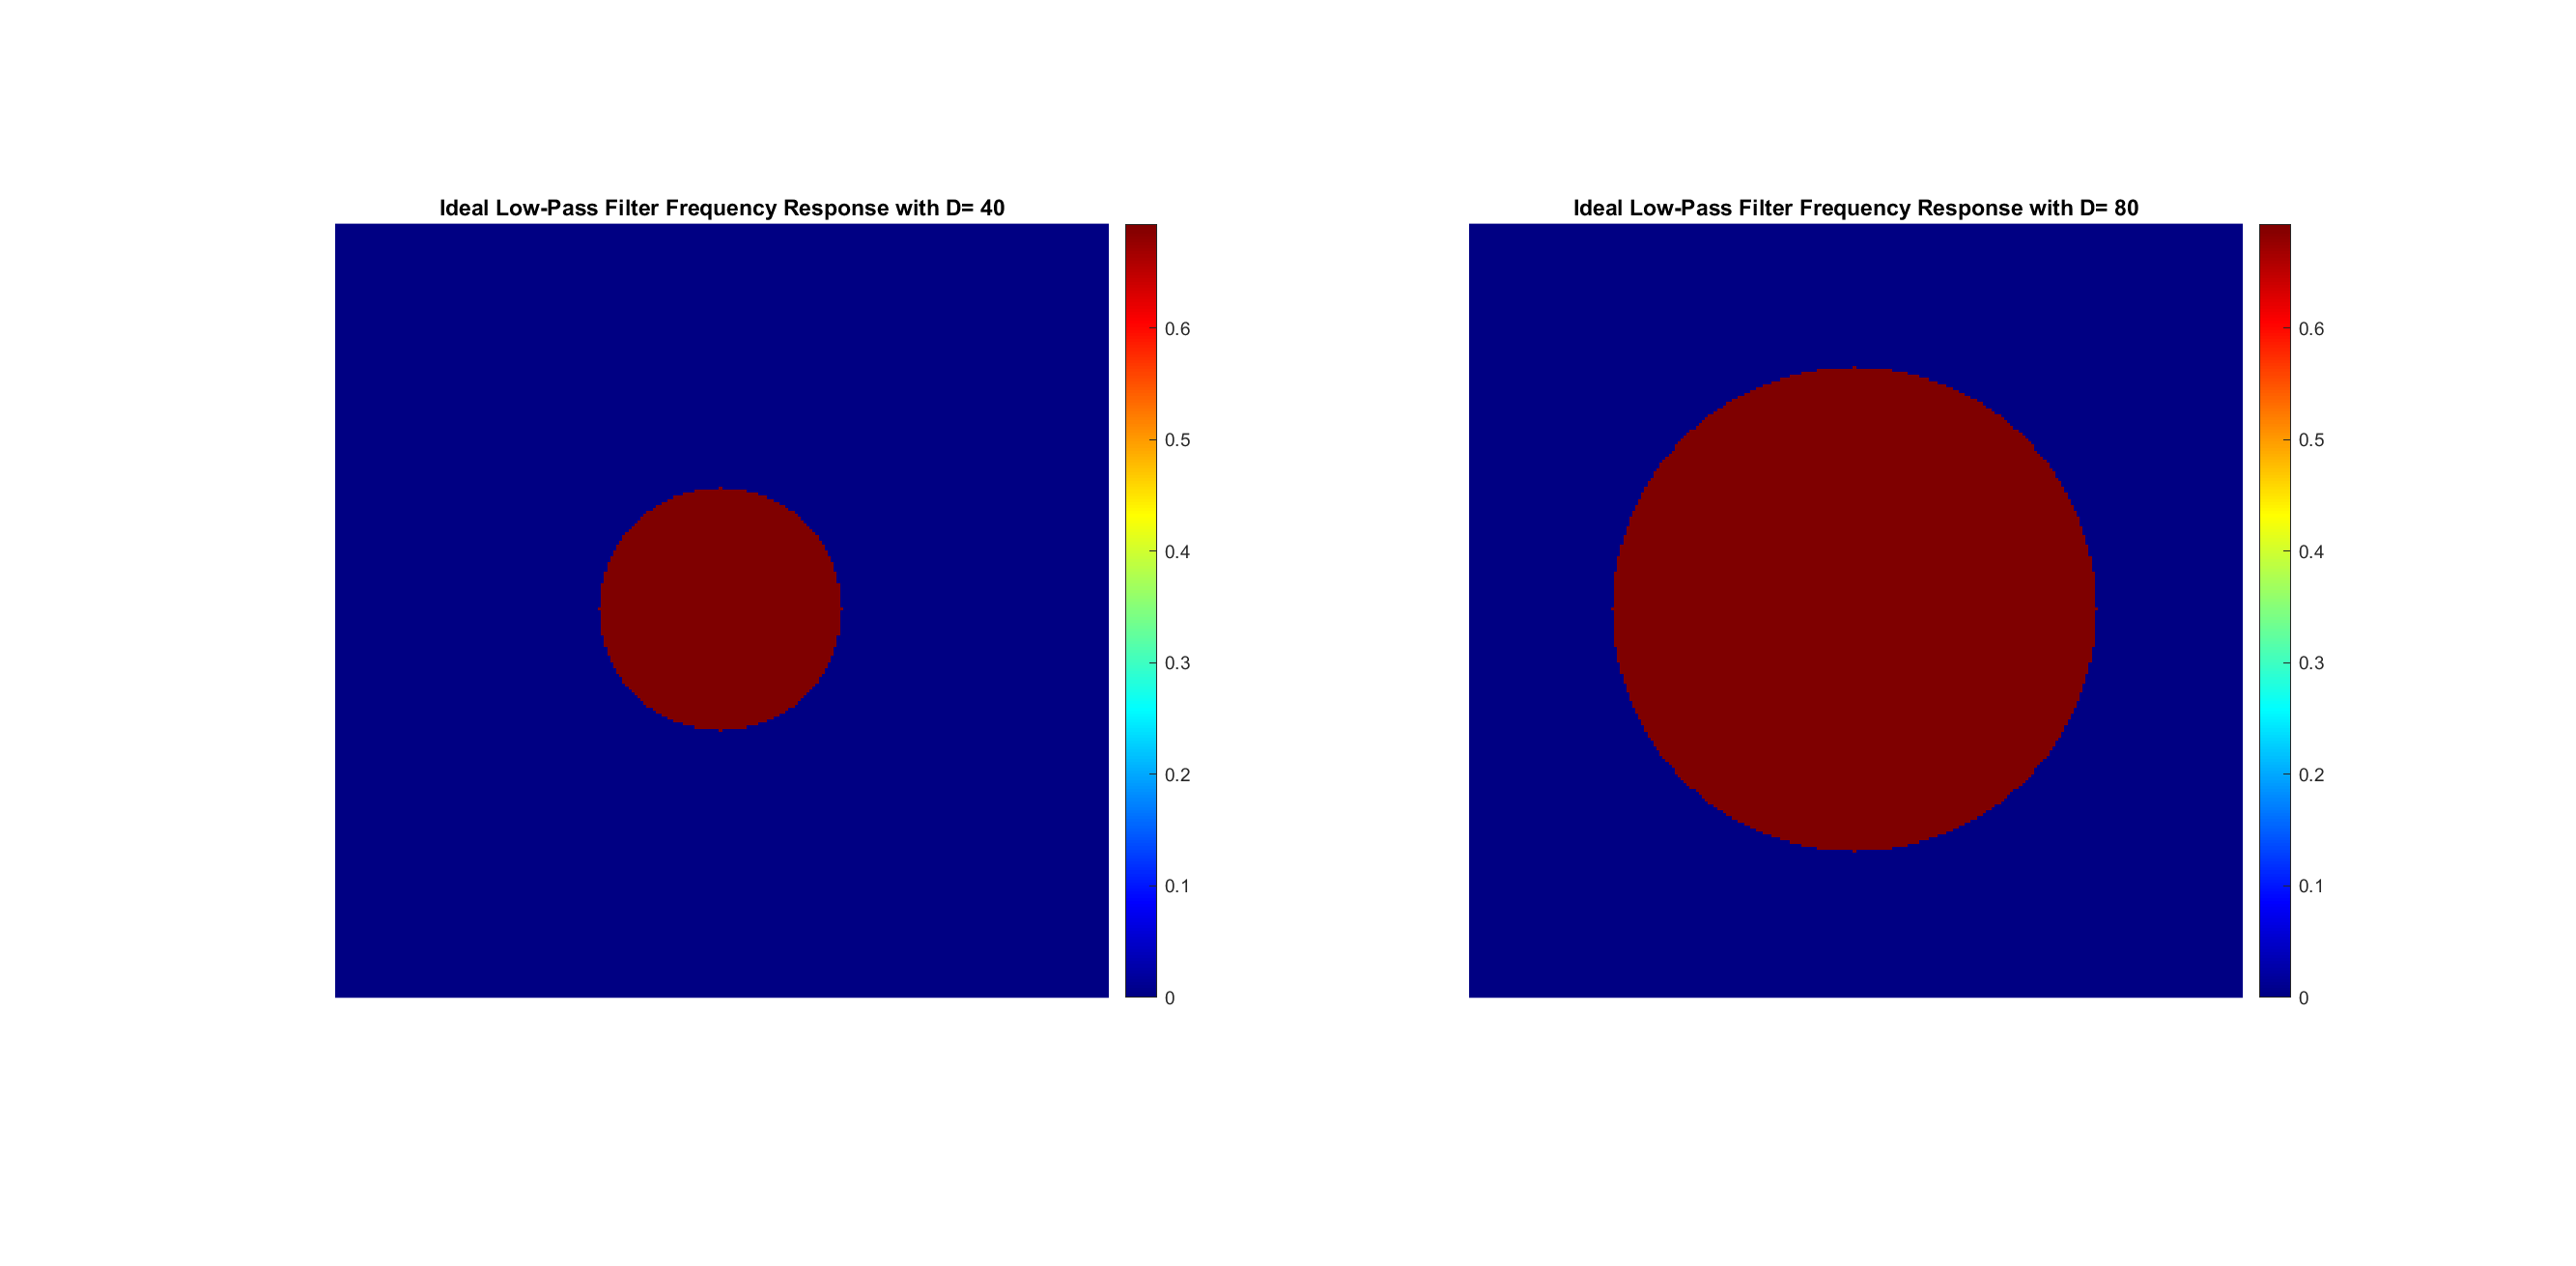
\includegraphics[width=.5\linewidth]{img3.png}
    \caption{Frequency Response of filters}
\end{figure}

The log absolute Fourier transform of the original and filtered images is as follows:
\begin{figure}[h]
    \centering
    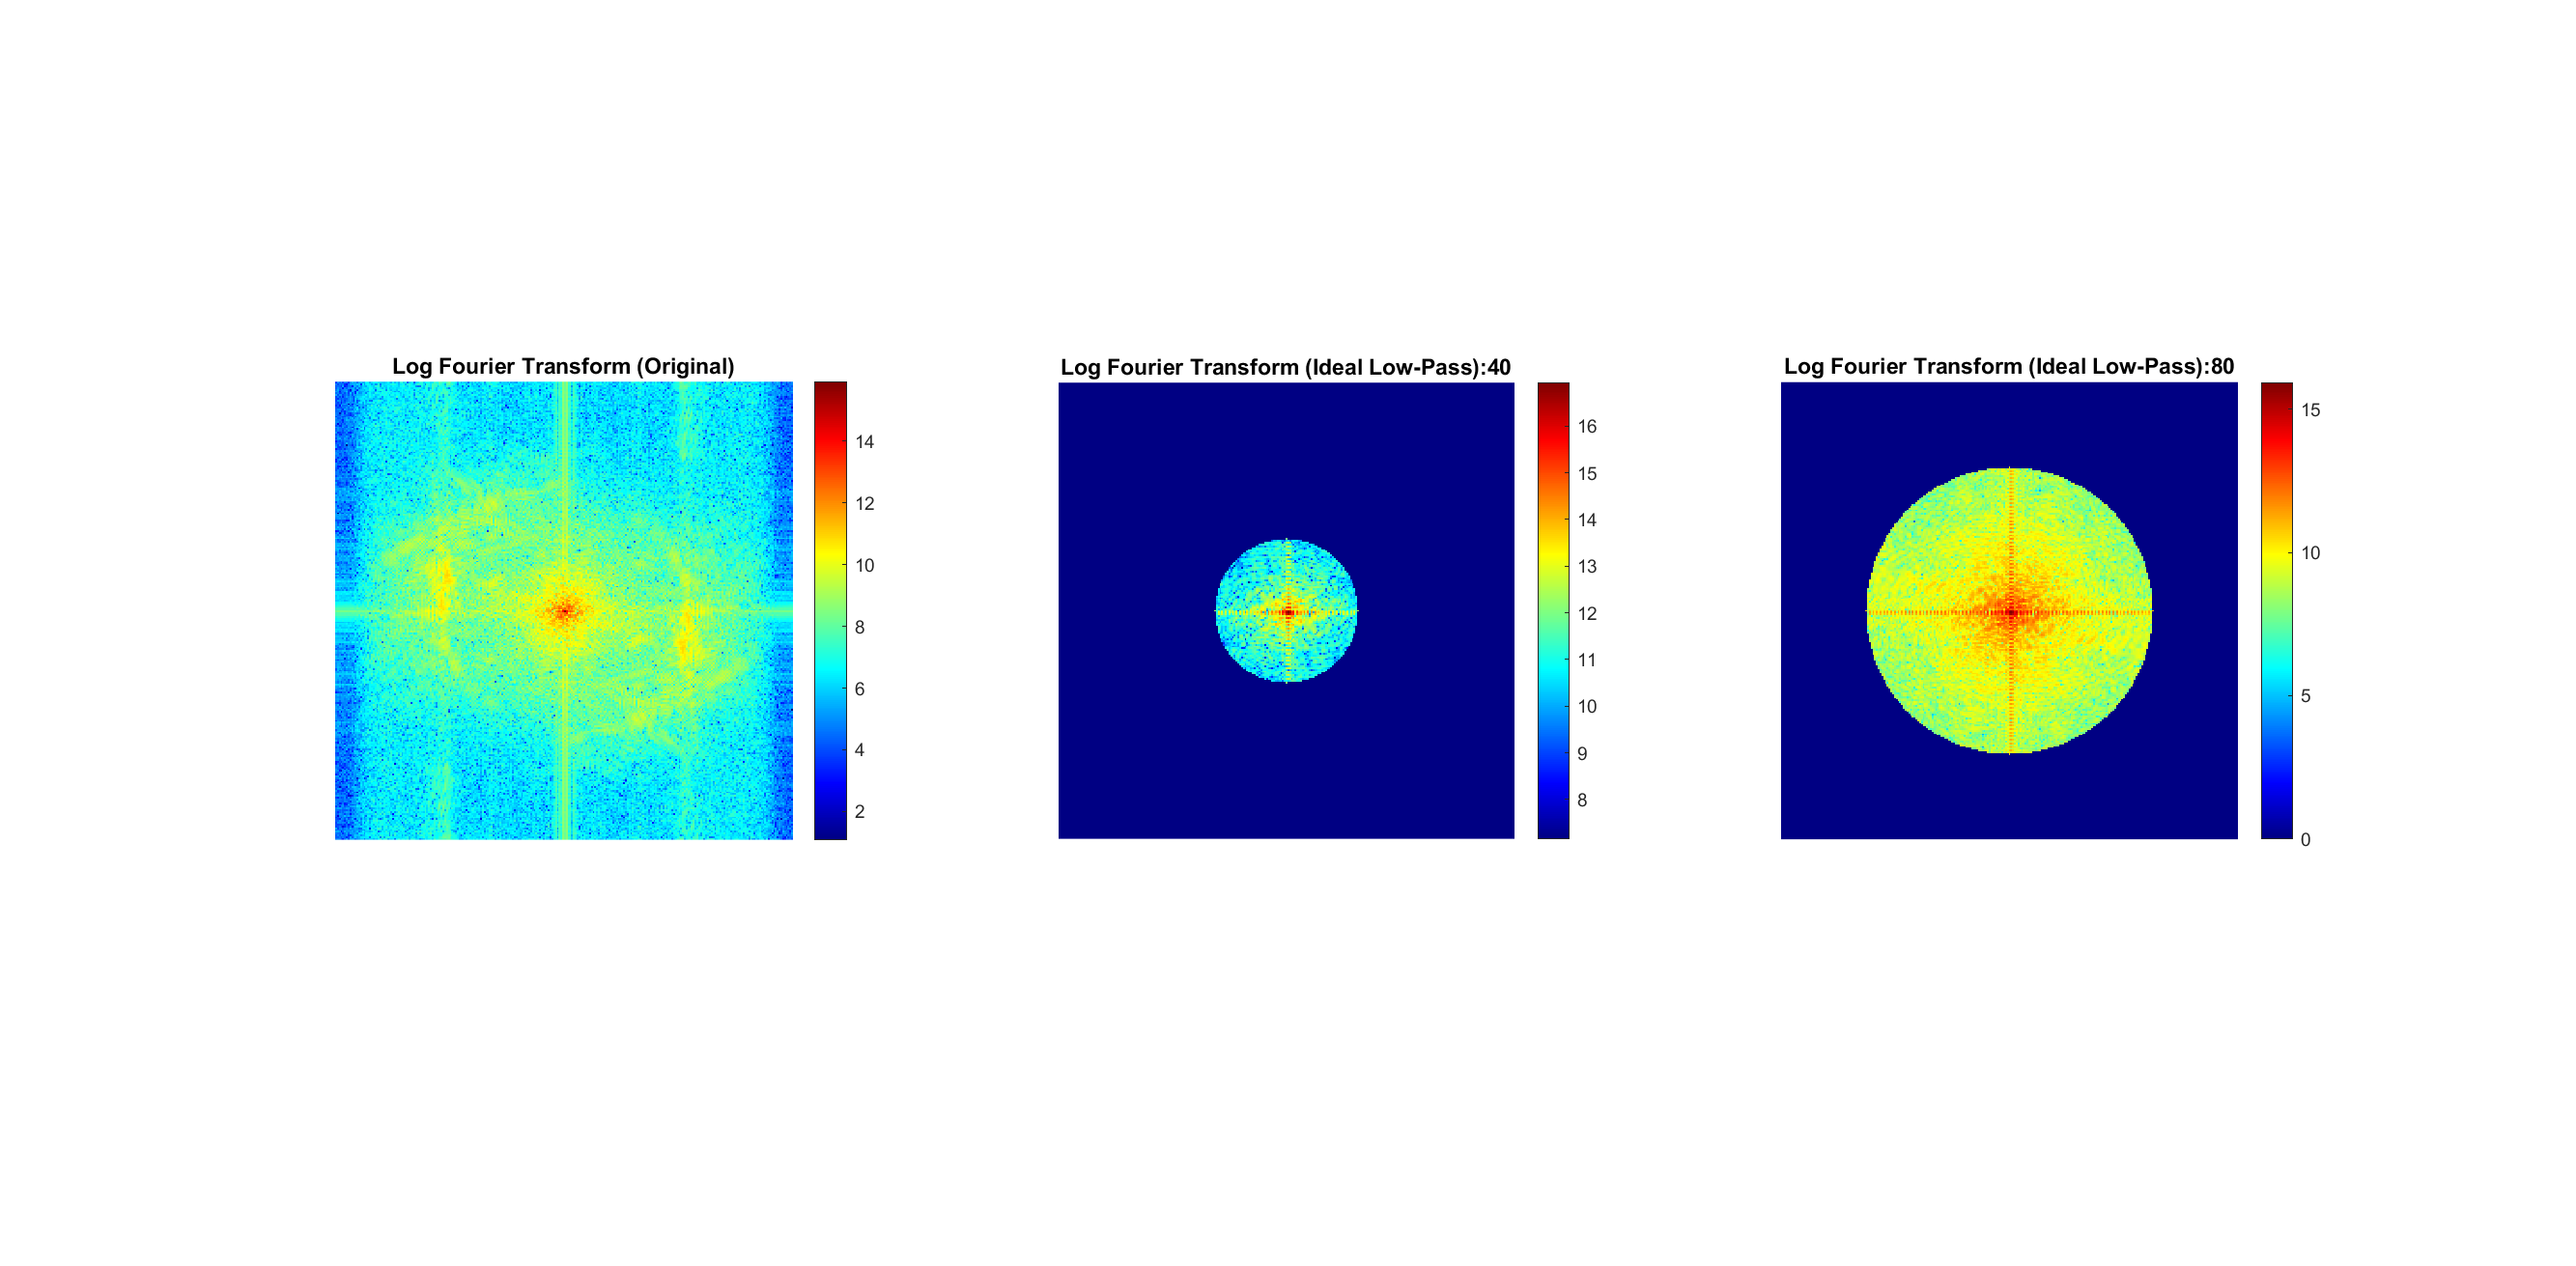
\includegraphics[width=\linewidth]{img2.png}
    \caption{Frequency Response of Origininal and Filtered Images}
\end{figure}

\subsection{Comments}
We observe that applying the low pass filter has a smoothing effect. This is because it gets rid of all the high-frequency components. Edges and fine textures, which are the high-frequency components are removed. We also observe the well-known ringing artifacts around the edges in the filtered images.
On observing the Fourier profile of the original and filtered image, we notice that all the frequencies outside the cutoff region have been eliminated for both values of D.


\section{Gaussian Low Pass filter}
In order to create a Gaussian low pass filter, we again create an empty image using the above method and find the Gaussian weights at each point according to the formula:
\[ H(u,v) = e^{-\frac{u^2 +v^2}{2\sigma^2}}\]

Please note that we have used the $\sigma$ parameter as applicable in the frequency domain according to above equation.
 
After appropriately padding both the original image and the filter, we calculated the Fourier transform of the image followed by performing a fftshift.
We then, point-wise multiplied the two images to receive the Fourier transform of the filtered image. After an ifftshift and ifft, we obtained the final filtered image. The output is plotted for the same.

\begin{figure}[h]
    \centering
    \begin{subfigure}{0.32\linewidth}
        \centering
        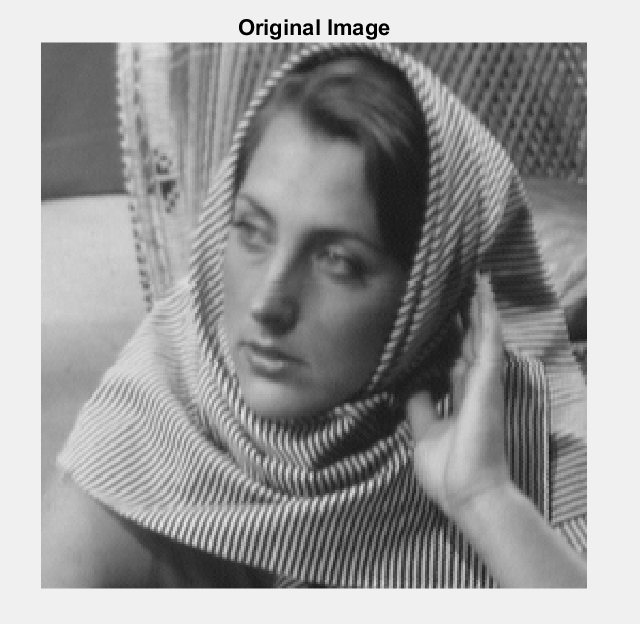
\includegraphics[width=\linewidth]{ori.png}
        \caption{Original Images}
    \end{subfigure}
    \begin{subfigure}{0.32\linewidth}
        \centering
        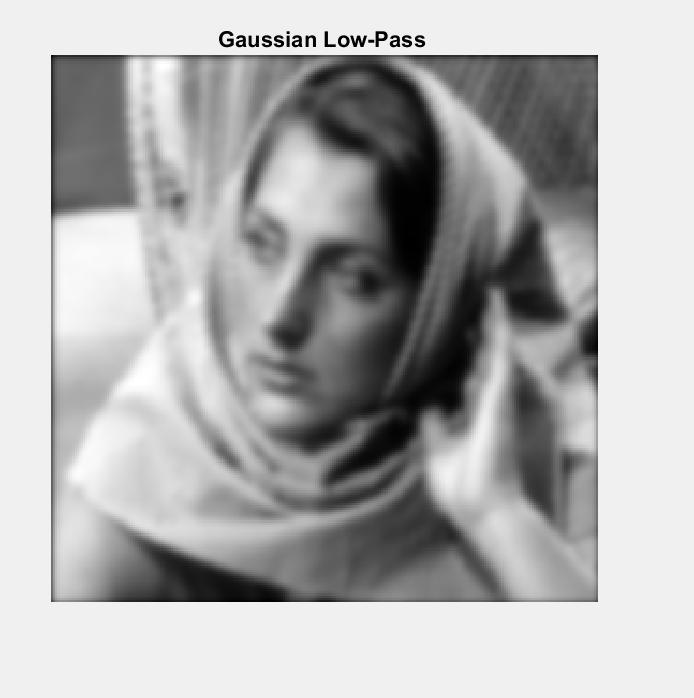
\includegraphics[width=\linewidth]{40_image.png}
        \caption{Gaussian Filtered Image with $ \sigma=40$}
    \end{subfigure}
    \begin{subfigure}{0.32\linewidth}
        \centering
        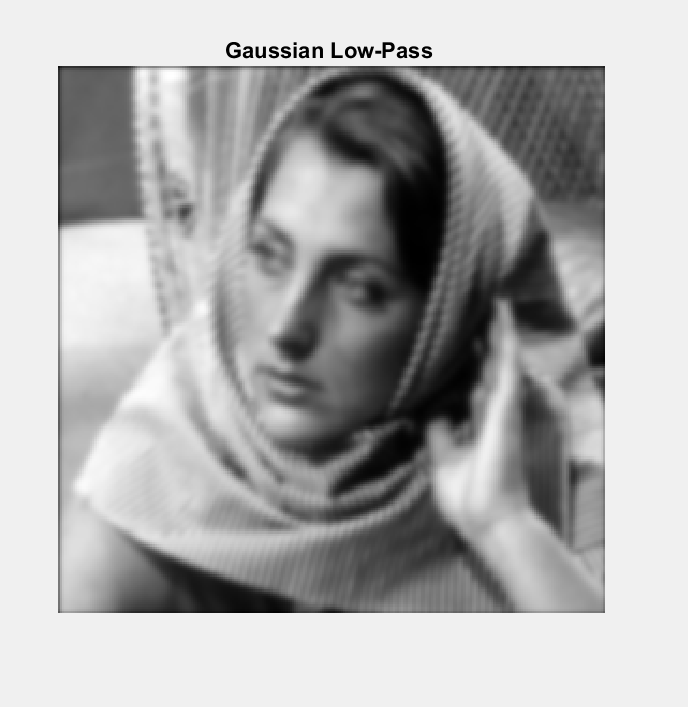
\includegraphics[width=\linewidth]{80_image.png}
        \caption{Gaussian Filtered Image with $ \sigma=80$}
    \end{subfigure}
    \caption{Barbara image}
    \label{fig:bo}
\end{figure}




\begin{figure}[h]
    \centering
    \begin{subfigure}{0.45\linewidth}
        \centering
        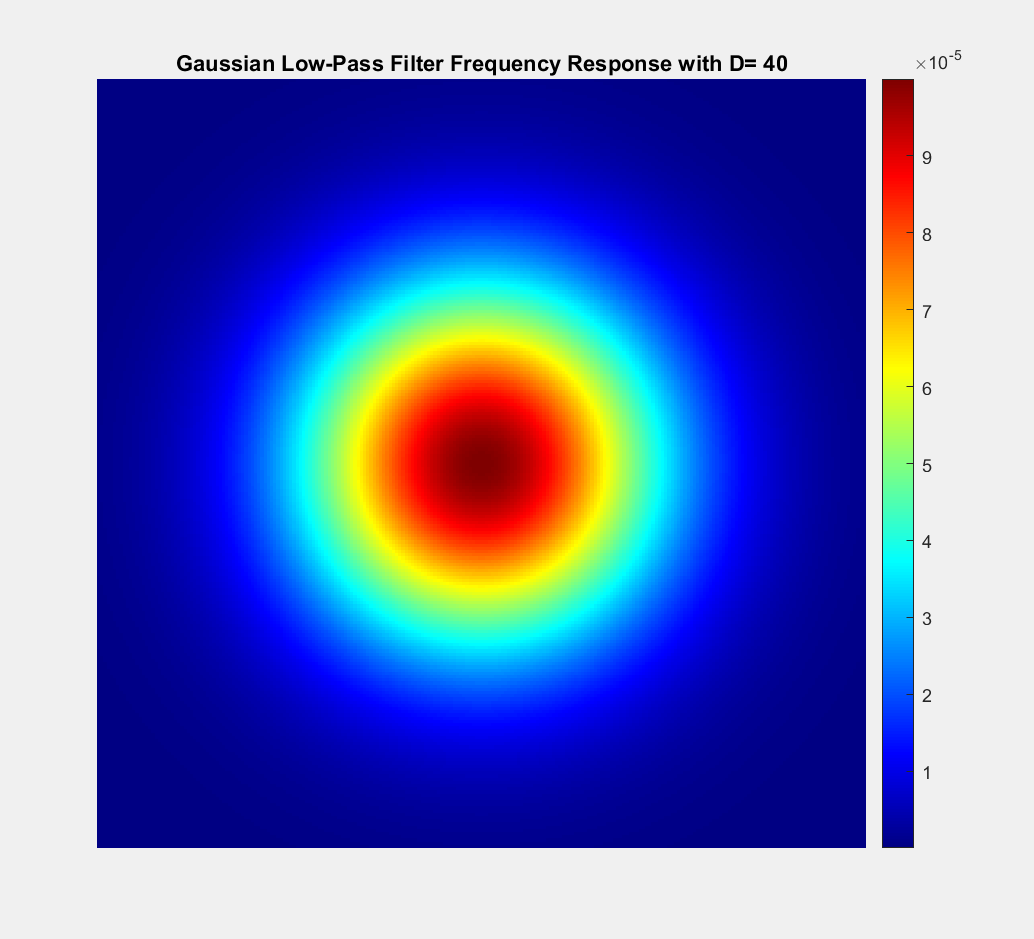
\includegraphics[width=\linewidth]{40_image_filter.png}
        \caption{Gaussian Filter with $\sigma = 40$}
    \end{subfigure}
    \begin{subfigure}{0.45\linewidth}
        \centering
        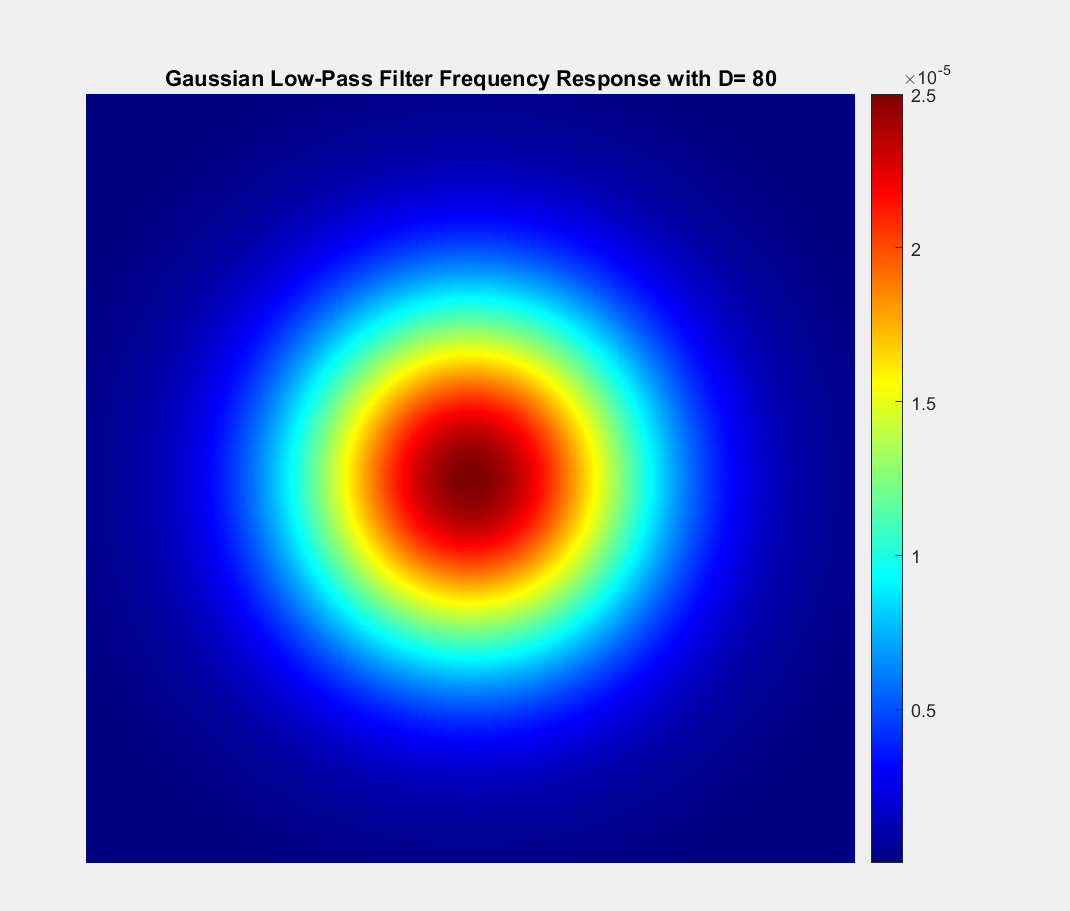
\includegraphics[width=\linewidth]{80_image_fil.png}
        \caption{Gaussian Filter with $\sigma = 80$}
    \end{subfigure}
    
    \caption{Plots of the Gaussian Filters}
    \label{fig:bo}
\end{figure}


\begin{figure}[h]
    \centering
    \begin{subfigure}{0.32\linewidth}
        \centering
        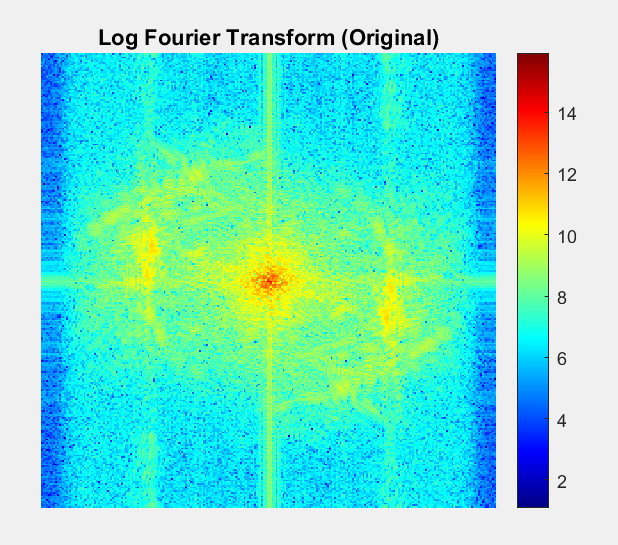
\includegraphics[width=\linewidth]{fo_ori.png}
        \caption{Original Image}
    \end{subfigure}
    \begin{subfigure}{0.32\linewidth}
        \centering
        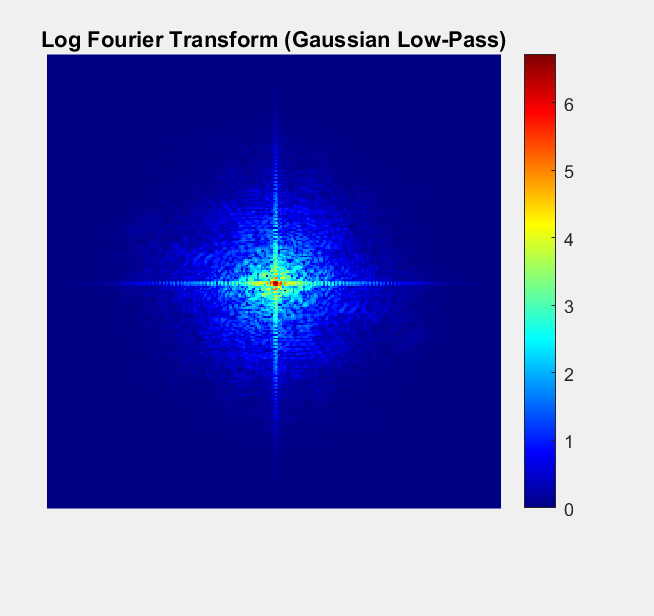
\includegraphics[width=\linewidth]{40_image_fo.png}
        \caption{Filtered Image with $ \sigma=40$}
    \end{subfigure}
    \begin{subfigure}{0.32\linewidth}
        \centering
        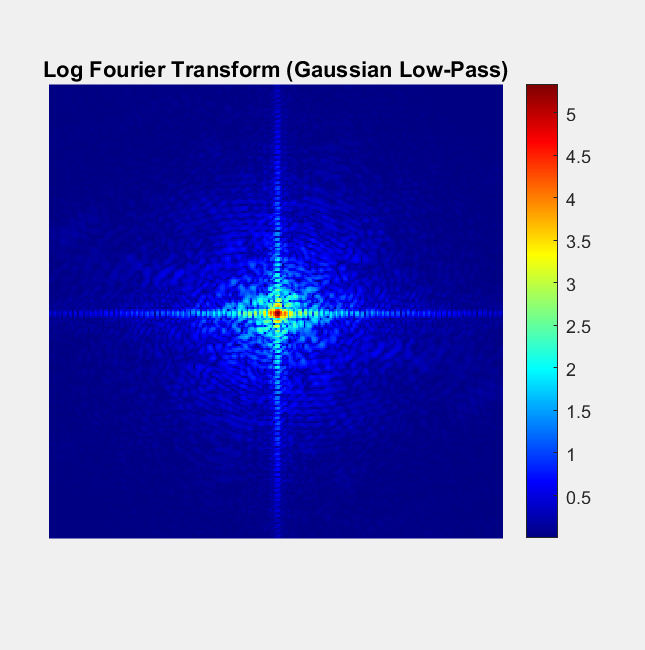
\includegraphics[width=\linewidth]{80_image_fo.png}
        \caption{Filtered Image with $ \sigma=80$}
    \end{subfigure}
    \caption{Plots of log of Fourier Response of Original and Filtered Images}
    \label{fig:bo}
\end{figure}

\subsection{Comments}
We observe that applying the Gaussian Filter has a smoothing effect. This is because it gets rid of all the high-frequency components. Edges and fine textures, which are the high-frequency components are removed Ringing artifacts are seen, which is in contrast to the ideal low-pass filter.

Also, as expected, the filters follow a Gaussian distribution and weaken the weightage of high-frequency components in the final image.

\section{Difference Between Ideal and Gaussian}
\subsection{Overall Image}
We observe the Ringing effect with an ideal low-pass filter, which is not observed in the Gaussian filter.
\subsection{Differences in Log of Absolute of  Fourier Transform}
In the case of the ideal filter, all frequencies above the cut-off are eliminated, for Gaussian only the weightage of high frequencies is reduced. With increasing D and $\sigma$, more and more frequencies are taken into account and hence we observe less smoothing with D= 80 and $\sigma = 80$ 
\subsection{Difference in Log of Absolute of Foruier of Filter}
We implemented an ideal filter, which in the frequency domain is just a circle of ones within a threshold and 0 otherwise. For higher D, the circle of allowed frequencies is larger.
We implemented a Gaussian Filter, which is the frequency domain that follows the Gaussian distribution.












    






\end{document}

